\documentclass[11pt]{article}
    \title{\textbf{Práctica Bloque 2}}
\author{Juan Miguel Pedrosa Garrido}
    \date{26 Octubre 2022}
    
    \addtolength{\topmargin}{-3cm}
    \addtolength{\textheight}{3cm}
\usepackage{graphicx}
\begin{document}

\maketitle
\thispagestyle{empty}

\section{Considera el lenguaje sobre el alfabeto \{a,b\} que solo contiene la cadena a}
Construye un AFD que reconozca el lenguaje y compruébalo con 6 cadenas.

Dado $M=(\{q_0,q_1,q_2\}, \{a,b\}, \delta, q_0, \{q_1\})$ es un DFA con:\\

\begin{table}[h!]
\begin{tabular}{c|c|c}
  $\delta(q,\sigma)$ & $a$ & $b$\\
  \hline
  $q_0$& $q_1$ & $q_2$\\
  \hline
  $q_1$& $q_1$ & $q_2$\\
  \hline
  $q_2$& $q_2$ & $q_2$
\end{tabular}
\end{table}
A continuación podemos ver la imagen de dicho autómata descrito anteriormente
\begin{figure}[htb]
	\centering
	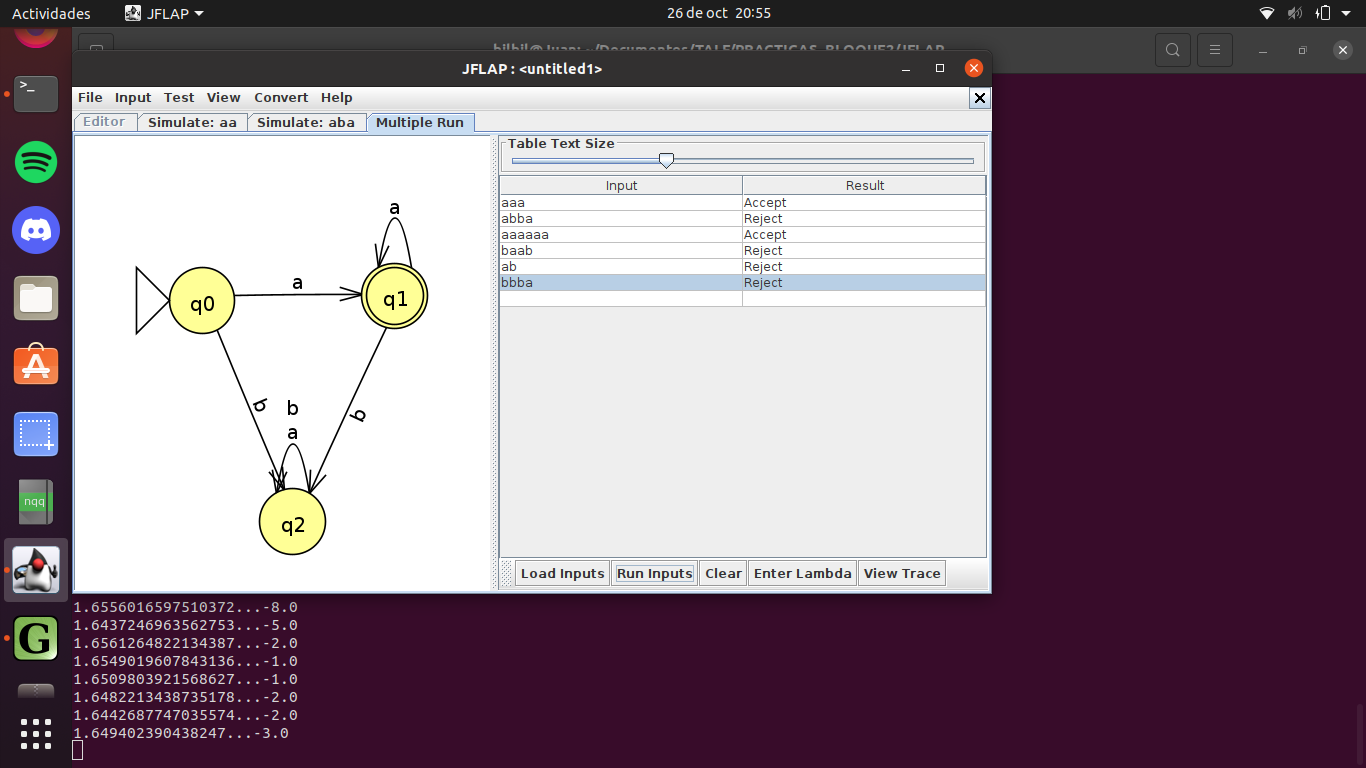
\includegraphics[width=1.25\textwidth]{1.png}
	\caption{Autómata finito determinista}
\end{figure}

\section{Comprueba la condición de bombeo para lenguaje independiente del contexto}

A continuación dejo las fotos de distintos testeos que hice con la herramienta del FCPC del JFLAP
\begin{figure}[htb]
	\centering
	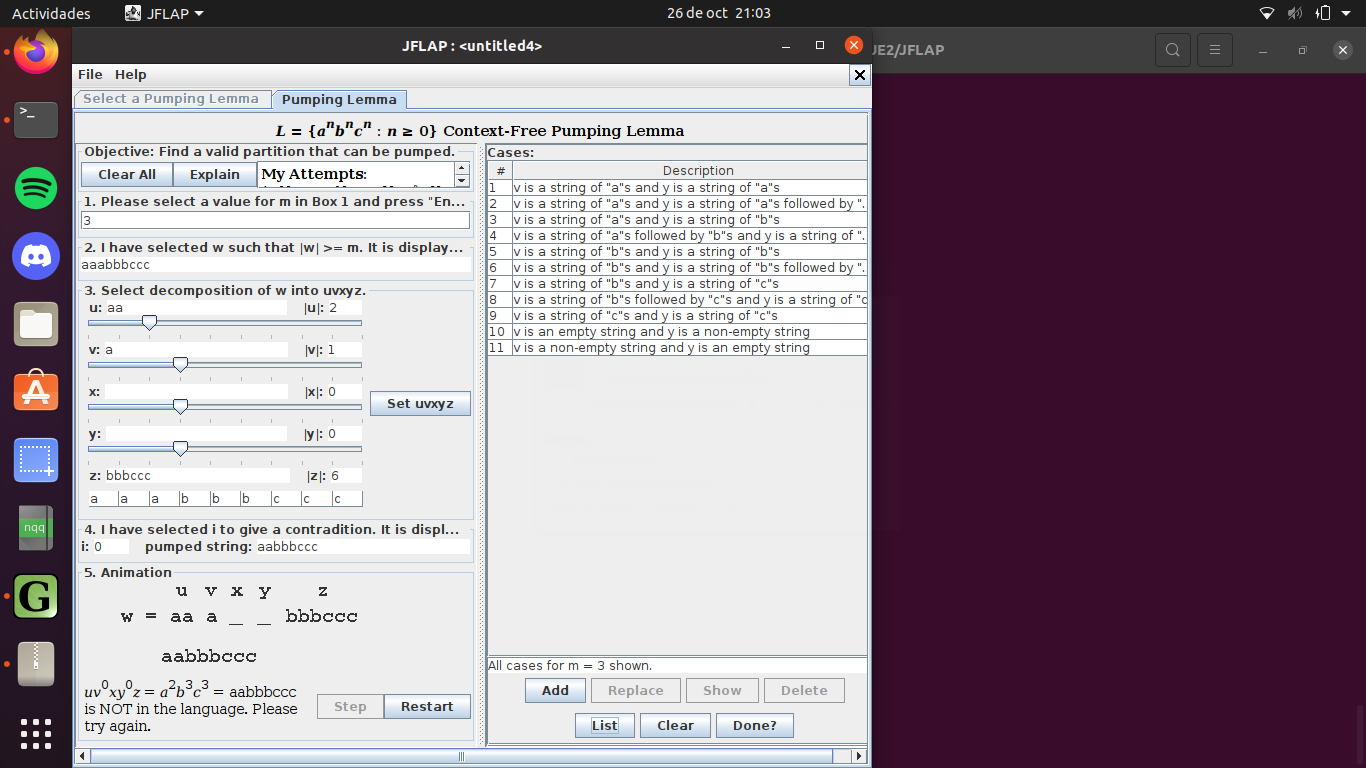
\includegraphics[width=0.75\textwidth]{3.1.png}
	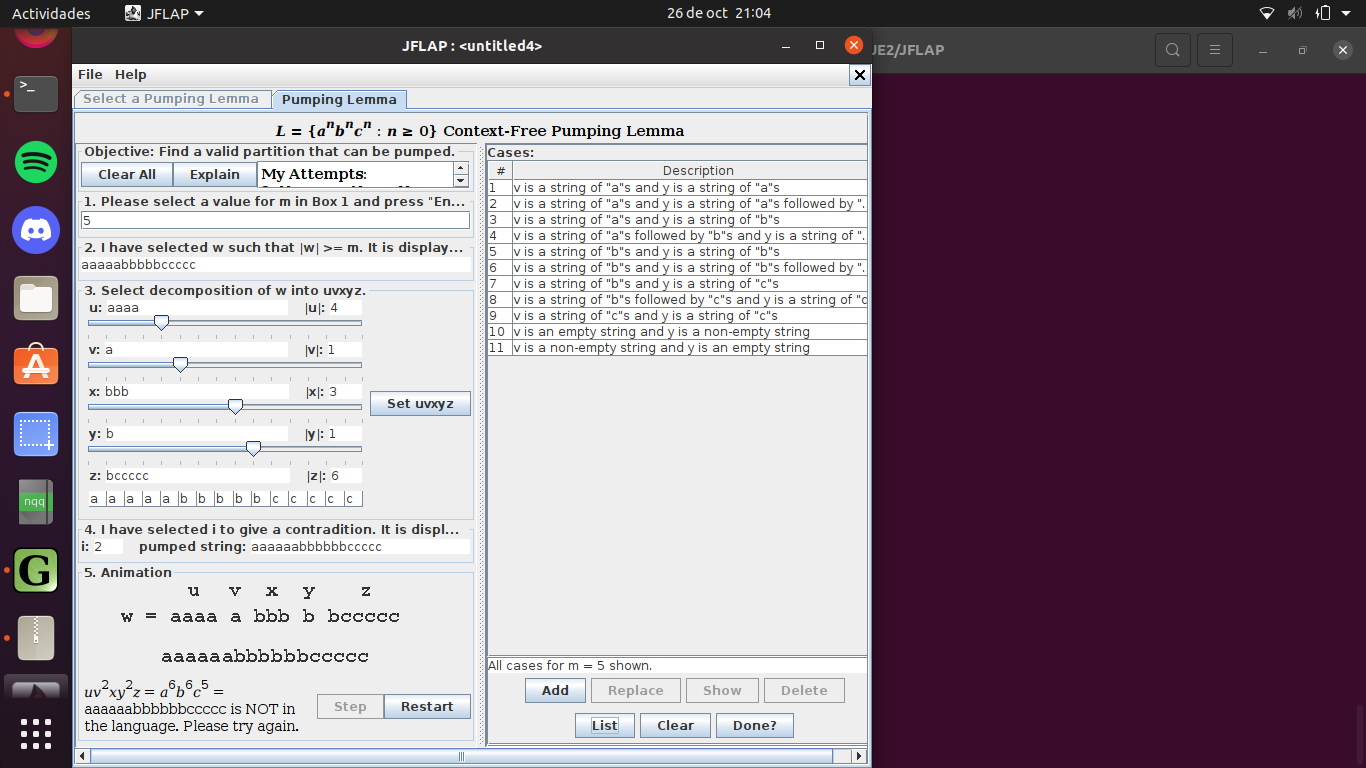
\includegraphics[width=0.75\textwidth]{3.2.png}
	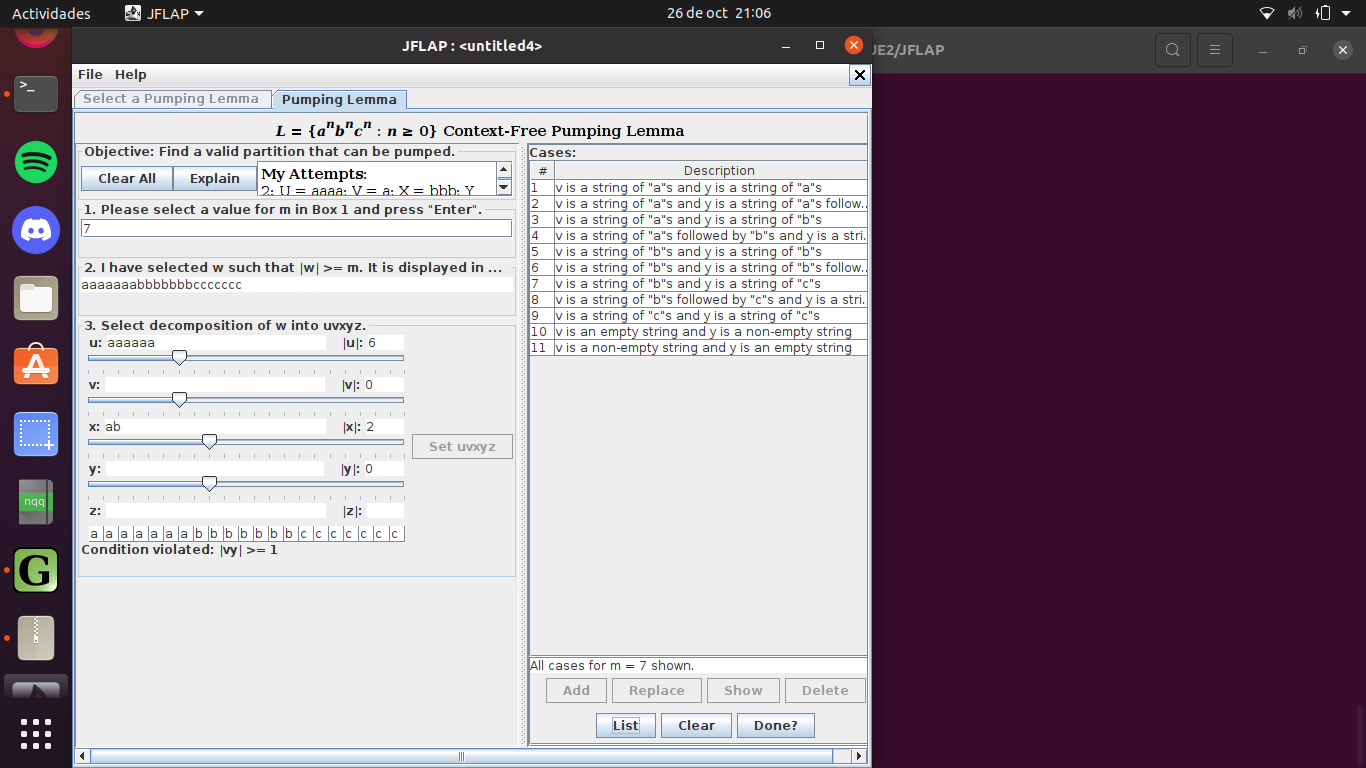
\includegraphics[width=0.75\textwidth]{3.3.png}
	\caption{Pruebas del testeo realizado con el FCPC}
\end{figure}

\section{Construir un APND que reconozca el lenguaje $L=\{0^n1²^n : n > 0\}$ }
A continuación, foto del autómata con pila creado
\begin{figure}[htb]
	\centering
	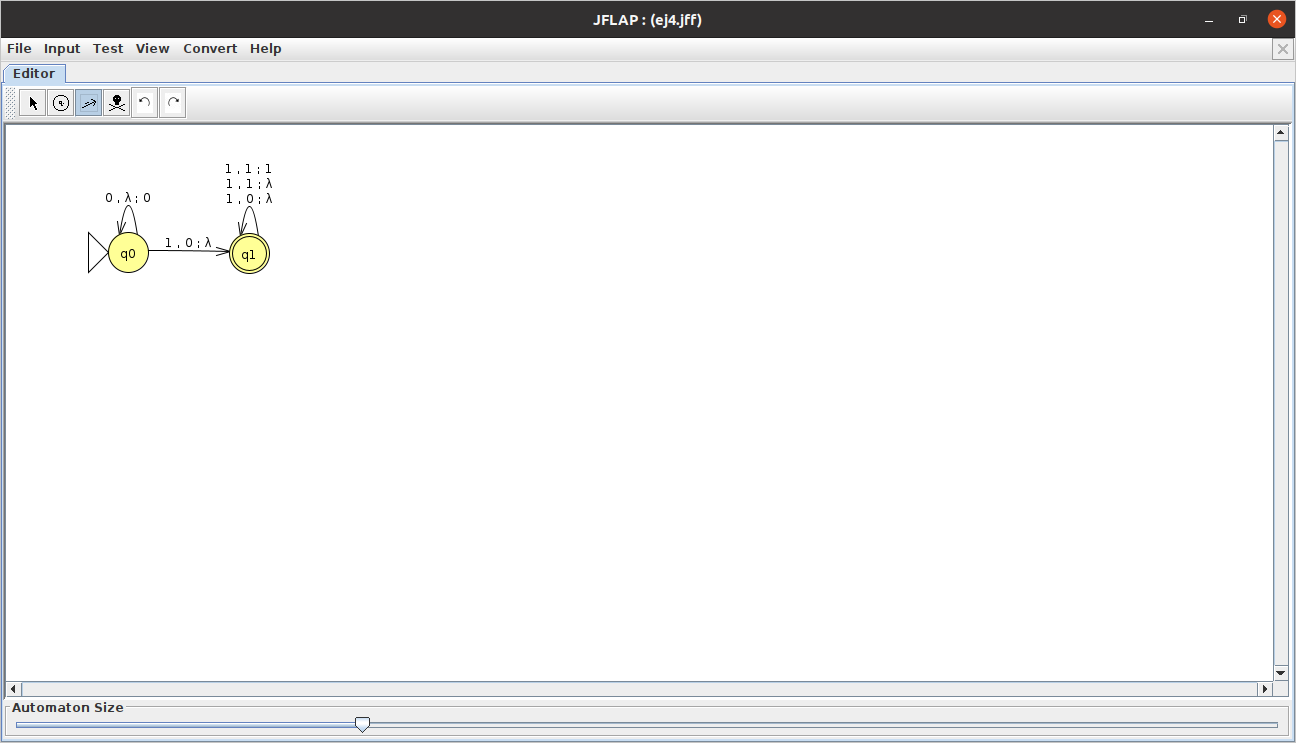
\includegraphics[width=1.25\textwidth]{4.png}
	\caption{Autómata con pila}
\end{figure}

\section{Describe el autómata del ejemplo 4.1.1}

Dado $M=(\{q_0,q_1,q_2\}, \{a,b\}, \delta, q_0, \{q_2\})$ es un DFA con:\\

\begin{table}[h!]
\begin{tabular}{c|c|c}
  $\delta(q,\sigma)$ & $a$ & $b$\\
  \hline
  $q_0$& $q_0$ & $q_1$\\
  \hline
  $q_1$& $q_2$ & $q_1$\\
  \hline
  $q_2$& $q_2$ & $q_0$
\end{tabular}
\end{table}


\end{document}

